\section{Introduction \& setup}
This guide shows how to install and use QEMU to run FreeRTOS.
\\QEMU is a free and open-source machine emulator and FreeRTOS is a real-time operating system kernel for embedded devices.
\\The guide primarily focuses on installing the necessary software components to set up an environment ready for replicating our experiments and system modifications involving FreeRTOS.

\subsection{What you need}

\begin{itemize}

    %\item First, you need to install the \textbf{FreeRTOS OS}, which is available for download here \url{https://www.freertos.org/a00104.html}. It's just a zip file with lots of customized versions of the OS for different boards. Once you download it, unzip it, and put it in an easily accessible directory.
    
    \item \textbf{QEMU}: it's a software that acts as an emulation system which allows to run a computer architecture (in our case ARM) within a different host environment (our machine).

    \item \textbf{GNU Arm Embedded Toolchain}: this is a set of open-source tools for developing software on ARM architecture-based processors. It is part of the GNU Compiler Collection (GCC) and includes various tools such as compiler, linker, assembler, debugger, and other utilities. 

    \item \textbf{gdb} (optional, only for debugging purpose): it's a powerful debugger for various languages which allows user to debug the code by stopping under conditions and by inspecting the state of the system.

    \item \textbf{make}: it's a widely used build automation tool in software development. It efficiently manages program compilation, recompiling only necessary parts when source code change. 

  \end{itemize}  

We divided the section according to the type of Host OS.

\subsubsection{ Linux users} \label{sec:LinuxUsers}

\begin{itemize}

    %\item First, you need to install the \textbf{FreeRTOS OS}, which is available for download here \url{https://www.freertos.org/a00104.html}. It's just a zip file with lots of customized versions of the OS for different boards. Once you download it, unzip it, and put it in an easily accessible directory.
    
    \item \textbf{QEMU}: To install it, execute the following command:
    \begin{minted}{bash}
        $ sudo apt install qemu-system-arm # for Ubuntu
    \end{minted}
     \begin{minted}{bash}
        $ sudo dnf install qemu-system-arm # for Fedora
    \end{minted}
     \begin{minted}{bash}
        $ sudo pacman -S qemu-system-arm # for ArchLinux
    \end{minted}

    \item \textbf{GNU Arm Embedded Toolchain}: You can look at the link \url{https://developer.arm.com/downloads/-/arm-gnu-toolchain-downloads}, or just run this command in the terminal:
    \begin{minted}{bash}
        $ sudo apt install gcc-arm-none-eabi # for Ubuntu
    \end{minted}
    \begin{minted}{bash}
        $ sudo dnf install arm-none-eabi-gcc arm-none-eabi-newlib # for Fedora
    \end{minted}
    \begin{minted}{bash}
        $ sudo pacman -S arm-none-eabi-gcc arm-none-eabi-newlib # for ArchLinux
    \end{minted}

    \item \textbf{gdb} (optional, only for debugging purpose): It's part of the Arm Toolchain so you can find it in the official website link of before: \url{https://developer.arm.com/downloads/-/arm-gnu-toolchain-downloads}, but we advice you to install it via these commands because the website binary have some issue.
    \begin{minted}{bash}
        $ sudo apt install gdb-multiarch
        $ sudo ln -s /usr/bin/gdb-multiarch /usr/bin/arm-none-eabi-gdb
        # for Ubuntu
    \end{minted}
    \begin{minted}{bash}
        $ sudo dnf install 'dnf-command(copr)'
        $ sudo dnf copr enable rleh/arm-none-eabi-gdb
        $ sudo dnf install arm-none-eabi-gdb 
        # for Fedora
    \end{minted}
    \begin{minted}{bash}
        $ sudo pacman -S arm-none-eabi-gdb # for ArchLinux
    \end{minted}

    \item \textbf{make}: Execute these commands in your terminal.
    \begin{minted}{bash}
        $ sudo apt install make # for Ubuntu
    \end{minted}
    \begin{minted}{bash}
        $ sudo dnf install make # for Fedora
    \end{minted}
    \begin{minted}{bash}
        $ sudo pacman -S make # for ArchLinux
    \end{minted}

  \end{itemize}  
\subsubsection{ Windows users} 

\begin{itemize}

\item \textbf{Windows Subsystem for Linux (WSL)}: a feature of Windows that allows you to run a Linux environment without the need for a separate virtual machine or dual-booting. We suggest you to use this tool to make your life easier as most of the commands used are based on Linux.
    \\Execute the following command in the PowerShell terminal:
    \begin{minted}{bash}
        $ wsl --install
    \end{minted}
   Any distribution works, the default one, and the one we used, is \textbf{Ubuntu}.
   Once you run the install command it will ask you to create username and password. Make sure you are in the WSL terminal, which should look like this:

    \begin{figure}[H]   % H is needed to show picture just above, instead of putting in other positions
        \centering
        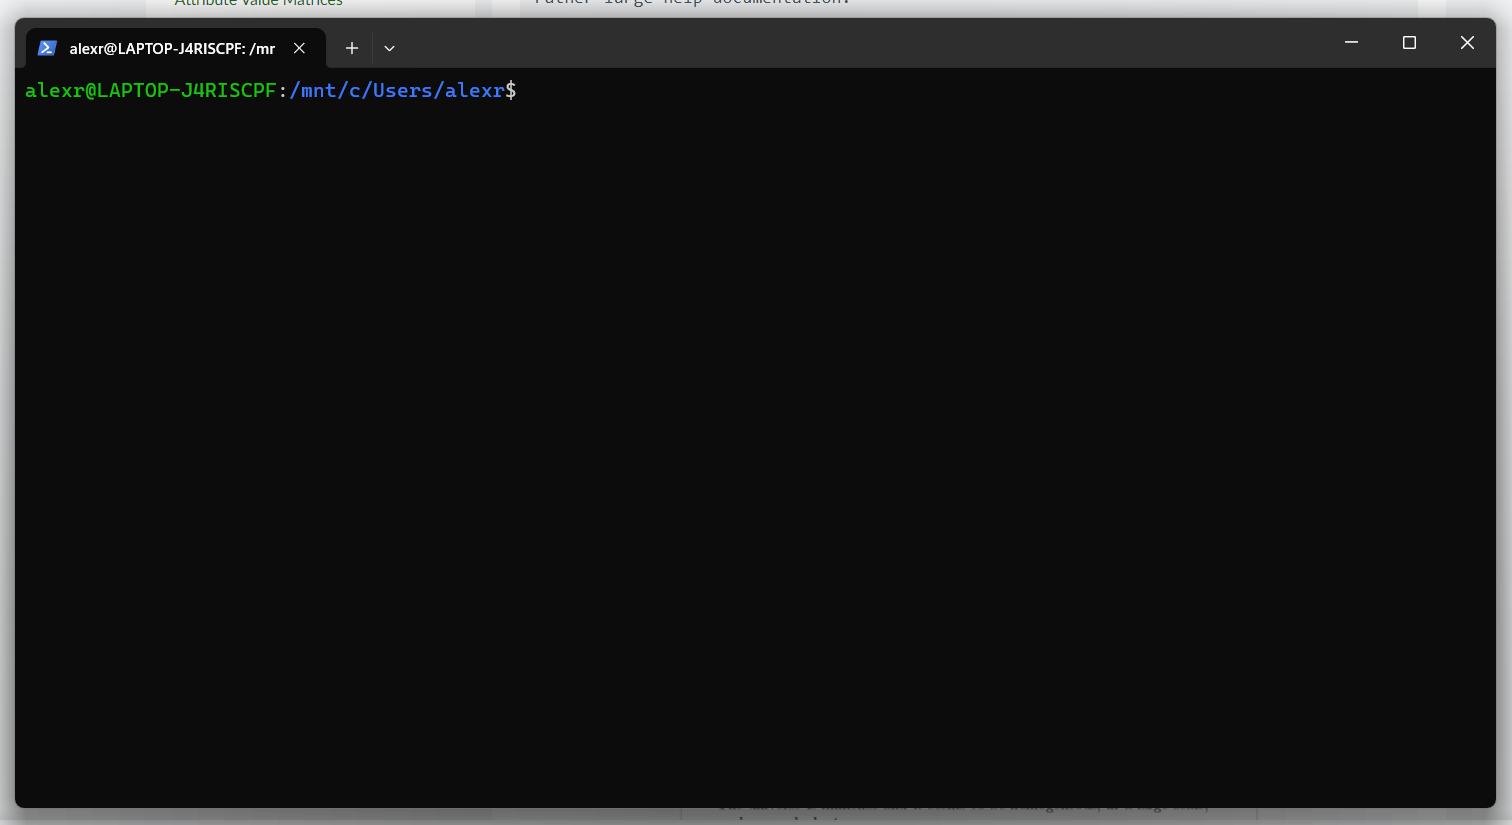
\includegraphics[scale=0.3]{Images/terminal.png}
        \caption{WSL terminal}
        \label{fig:enter-label}
    \end{figure}

    Then just follow the Ubuntu steps above in \ref{sec:LinuxUsers}.

\end{itemize}


\subsubsection{ Mac users} 


\begin{itemize}

\item \textbf{QEMU}: you can get QEMU through Homebrew. If it's not already installed, install Homebrew following this link \url{https://brew.sh}, then run:
\begin{minted}{bash}
        $ brew install qemu
    \end{minted} 
\item\textbf{GNU Arm Embedded Toolchain}: to download it you can look at the link \\\url{https://developer.arm.com/downloads/-/arm-gnu-toolchain-downloads}
\end{itemize}
\begin{itemize}
\item\textbf{make}: to install it run: 
\begin{minted}{bash}
        $ brew install make
    \end{minted}
    
\item\textbf{gdb} (optional,only for debugging purpose): to install it run: 
\begin{minted}{bash}
        $ brew install gdb
    \end{minted}

\item\textbf{C++} (through Xcode Command Line Tools) to install it run:
\begin{minted}{bash}
        $ xcode-select --install
    \end{minted}
\end{itemize}   
To make the ARM compiler globally accessible on your system, you need to add the compiler's path to the 'PATH' environment variable. This can be achieved using the following command in the terminal:
\begin{minted}{bash}
        $ export PATH="/path/to/arm-compiler/bin:$PATH"
    \end{minted}
Replace "/path/to/arm-compiler" with the actual path where your ARM compiler is installed. This command appends the ARM compiler's path to the 'PATH variable'. When the 'PATH' variable is queried, the system will now include the ARM compiler's path, allowing you to execute commands like arm-none-eabi-gcc from any directory in the terminal.
In the same way to include the QEMU emulator in your shell's PATH, use the following command:
\begin{minted}{bash}
        $ export PATH="/path/to/qemu-system-arm:$PATH"
\end{minted}
It's important to note that those modifications are temporary for the current terminal session. If you want to make this change permanent, you can add it to the configuration file of your terminal profile, such as .bashrc or .zshrc depending on your shell.

\subsection{ Next steps }
Now that we have the required tools, let's go ahead and clone the Git repository.\\
To use a specific branch, choose the desired branch from the list provided in the README, available at the following link:\url{https://baltig.polito.it/caos2023/group36/-/blob/master-update/README.md}. \\This ensures that you are using  the intended branch. Then you can clone the branch repository running:
\begin{minted}{bash}
           $ git clone -b NAME_BRANCH https://baltig.polito.it/caos2023/group36

    \end{minted}
In the folder you will find the makefile. This GCC project, in fact, uses a simple makefile that can be built from the command line.
\\\\Make sure you are in the correct folder and proceed by executing the 'make' command.
\begin{minted}{bash}
           $ make
    \end{minted}
%insert the image here

\leavevmode\\Next, proceed by launching QEMU emulator with the following command:
\begin{minted}{bash}
           $ qemu-system-arm -machine mps2-an385 -cpu cortex-m3 -kernel 
           output/RTOSDemo.out -monitor none -nographic -serial stdio
\end{minted}

\begin{itemize}
    \item -machine and -cpu allow us to emulate a specific machine and CPU. In our case, we are emulating an MPS2-AN385 board equipped with a Cortex-M3 CPU.
    \item -kernel is used to specify our compiled OS in the form of ELF file.
    \item -serial stdio lets us to attach our terminal to the serial UART peripheral.
    \item -nographic is used to disable graphical output, making QEMU a simple command-line application.
    \item -monitor none is employed to avoid having the QEMU monitor console, as it is unnecessary due to the use of -nographic, which prevents console access in any case.
\end{itemize}

